\chapter{Distributed Safe Bayesian Optimization}
\label{ch:distbo}


This chapter considers the problem of distributing the safe optimization process to multiple computing nodes. We are creating hyperspaces from the given optimization search space to achieve this. We successively divide the search space into new hyperspaces and deploy them to new computing nodes till we reach a leaf hyperspace. Division of search space will happen as a new safe point evaluated in non-deployed hyperspace. An extension of this work considers the overlapped hyperspace, where we share the points evaluated in the overlapped region with corresponding nodes. We also discussed the software implementation of the system. Furthermore, at last, we explained the search space division to create hyperspace with an example.

\section{System Model and Problem Statement}
\par We will be given with an unknown function $f: \mathcal{X} \to \mathbb{R}$ over some domain $\mathcal{X} \subset \mathbb{R}^d$. But $f$ is expensive to compute and no access to gradients.
The objective\textcolor{white}{i}of the\textcolor{white}{i}safe optimization problem\textcolor{white}{i}is to find the maximum\textcolor{white}{i}of an unknown function $f(x)$ where $x \in \mathcal{X}$ subject to\textcolor{white}{i}safety constraints. 
We assume that $f(x)$ is a Lipschitz continuous function of $x$ on a compact set $\mathcal{X}$. The Lipschitz\textcolor{white}{i}constant is\textcolor{white}{i}assumed to be $L$.
Furthermore, the seed set $S_0 \subset \mathcal{X}$ that contains atleast one safe point. 
We should ensure that, for all time steps $t$, it holds that $f(x_t) \geq h$, where $h$ is a problem-specific safety threshold.
We can divide each search space dimension into $n$ number of subspaces and take the all possible combinations to form $n^d$ hyperspaces. Thus we assume that there are $m \ge n^d$ computing nodes avialable. 
Additionally, we will be having time and communication constraint for a given network connection.
\par We\textcolor{white}{i}note that since the\textcolor{white}{i}function is unknown, we optimize the\textcolor{white}{i}function by observing\textcolor{white}{i}the value of the function at points $x_t \in \mathcal{X}$ which are chosen\textcolor{white}{i}for every\textcolor{white}{i}time $t$, meeting the safety constraint $f(x_t) \geq h$.
So our problem is to find safely reachable point $x^* \in \mathcal{X}$ which maximizes the value of our unknown function $f$, by distributing the computation possibly among $m$ nodes by successively dividing and then deploying each safely reachable hyperspace into each node.

\section{Distributed SafeOpt}
\label{sec:dsbo}
For a given search space $\mathcal{X}$ with $d$ search dimensions(parameters) and $n$ number of subspaces per parameter, we can take the all possible combination of subspaces to create hyperspaces. So $n^d$ hyperspaces are possible. 
We start the optimization process in a single node for a given objective function $f$, search space $\mathcal{X}$ with safe set $S_0$. 
We take the hyperspace in which initial safe points of set $S_0$ belong as the \textit{currently deployed hyperspace}. 
As the next step of the optimization process, we will get the point $x_{next}$ for objective function evaluation.
We check the function value $f(x_{next}) \geq h$ for safety constraint violation. 
Also, if the point is safe, check whether the point $x_{next}$ belongs to the new non-deployed hyperspace for the sampled new point. 
The points that do not meet the safety constraint are considered unsafe evaluations and stored in the \textit{all evaluated points} array. Furthermore, we will use this array to define prior to the upcoming search space deployment after splitting the search space.
The point that meets safety constraints and is present in new non-deployed hyperspace splits the present search space into \textit{current-hyperspace} and \textit{new-hyperspace}. 
The point $x_{next}$ will be the initial safe seed for the new search space that defines \textit{new-hyperspace}, and we start an optimization process for this \textit{new-hyperspace} in a new node. 
The $S_0 \cup \{ \text{any other safe point evaluated in }\textit{current-hyperspace } \}$ will be the safe seed for other search space that defines \textit{current-hyperspace} and the optimization process will be continued in the same node with updated search space bounds. 
Above mentioned procedures will be repeated to successively divide the search space into a leaf hyperspace (leaf node). 

Algorithm \texttt{DistributedSafeOpt}\ref{alg:dsbo} explains the initialization of the optimization process into a node, and algorithm \texttt{DeployHyperspace}\ref{alg:deployhs} recursively instantiates the new optimization process into new nodes. Optimization process in each node uses \texttt{SafeOpt} \ref{alg:safeopt} for safe optimization. An abstract architecture of the software implementation and an example showing how hyperspaces are created is discussed in the following subsections.

\begin{algorithm}[h!]
%	\SetAlgoVlined
	\caption{\texttt{DistributedSafeOpt}}
	\label{alg:dsbo}
	\KwIn{Objective function $f$, GP prior($\mu, k$), Domain $\mathcal{X} \subset \mathbb{R}^d$, Number of subspaces per dimension $n$, Safe seed set $S_0$, Safety threshold $h$, Evaluation contraint $L$}
	\ForEach{$searchDimension$ in $\mathcal{X}$}
	{
		divide $searchDimension$ into $n$ subspaces.
	}
	Take all possible combinations of subspaces to form $hyperspaces$. $(n^d)$\\
	$currentSafeHyperspace = hyperspace | S_0 \in hyperspace$\\
	Initially deploy optimization process for whole search-space into a single node.\\		
\end{algorithm}

\begin{algorithm}[h!]
%	\SetAlgoVlined
	\caption{\texttt{DeployHyperspace}}
	\label{alg:deployhs}
	\KwIn{$f$, GP($\mu, k$), $\mathcal{X}$, $S_0$, $h$, $L$, $currentSafeHyperspace$, }
	Initialize \texttt{SafeOpt} with safe seed points $S_0$.\\
	\If{currentSafeHyperspace $is$ leafHyperspace}
	{
		\While{$L>0$}
		{
			$newPoint=$ \texttt{SafeOpt}.optimize()\\
			$funcValue=f(newPoint)$\\
			add $(newPoint,funcValue)$ to $S_0$\\
		}
		\KwRet{}
	}
	\While{$L>0$}
	{
		$newPoint=$ \texttt{SafeOpt}.optimize()\\
		$funcValue=f(newPoint)$\\
		add $(newPoint,funcValue)$ to $S_0$\\
		$newSafeHyperspace = hyperspace | newPoint \in hyperspace$\\
		\eIf{$funcValue \ge h$ \textbf{AND} $newSafeHyperspace \neq currentSafeHyperspace$}
		{
			Split the search-space between two hyperspaces into $newSearchSpace$ and $currentSearchSpace$.\\
			Call \texttt{DeployHyperspace} for $newSearchSpace$ corresponding to $newSafeHyperspace$ to new worker node.\\
			Update the current worker node's search-space to $currentSearchSpace$ corresponding to $currentSafeHyperspace$ and continue optimization process.\\
		}
		{
			add $(newPoint,funcValue)$ to \texttt{SafeOpt} model.\\
		}
	}
\end{algorithm}

\clearpage
\subsection{Implementation Details}
\label{subsec:dsbo-impl}

To distribute the workload among multiple computing nodes, we are using \texttt{RAY} \cite{ray.framework} framework. \texttt{RAY} provides an application-level API called \textit{Actor}, a stateful process that executes, when invoked, only the methods it exposes. Figure \ref{fig:dsbo-architecture} shows the abstract representation of the implementation.

A driver program starts the optimization process by instantiating a \textit{Shared Data} actor, which will \textit{create hyperspaces} from the search space \textit{bounds} and the number of subspaces asked to form for each dimension. It also creates the required data structures to keep the information about the hyperspace deployment status. It also maintains a list that holds \textit{all points evaluated} by all nodes. This list serves as a prior for deploying the new optimization processes.

\begin{figure}[h!]
	\centering
	\hspace*{-5em}
	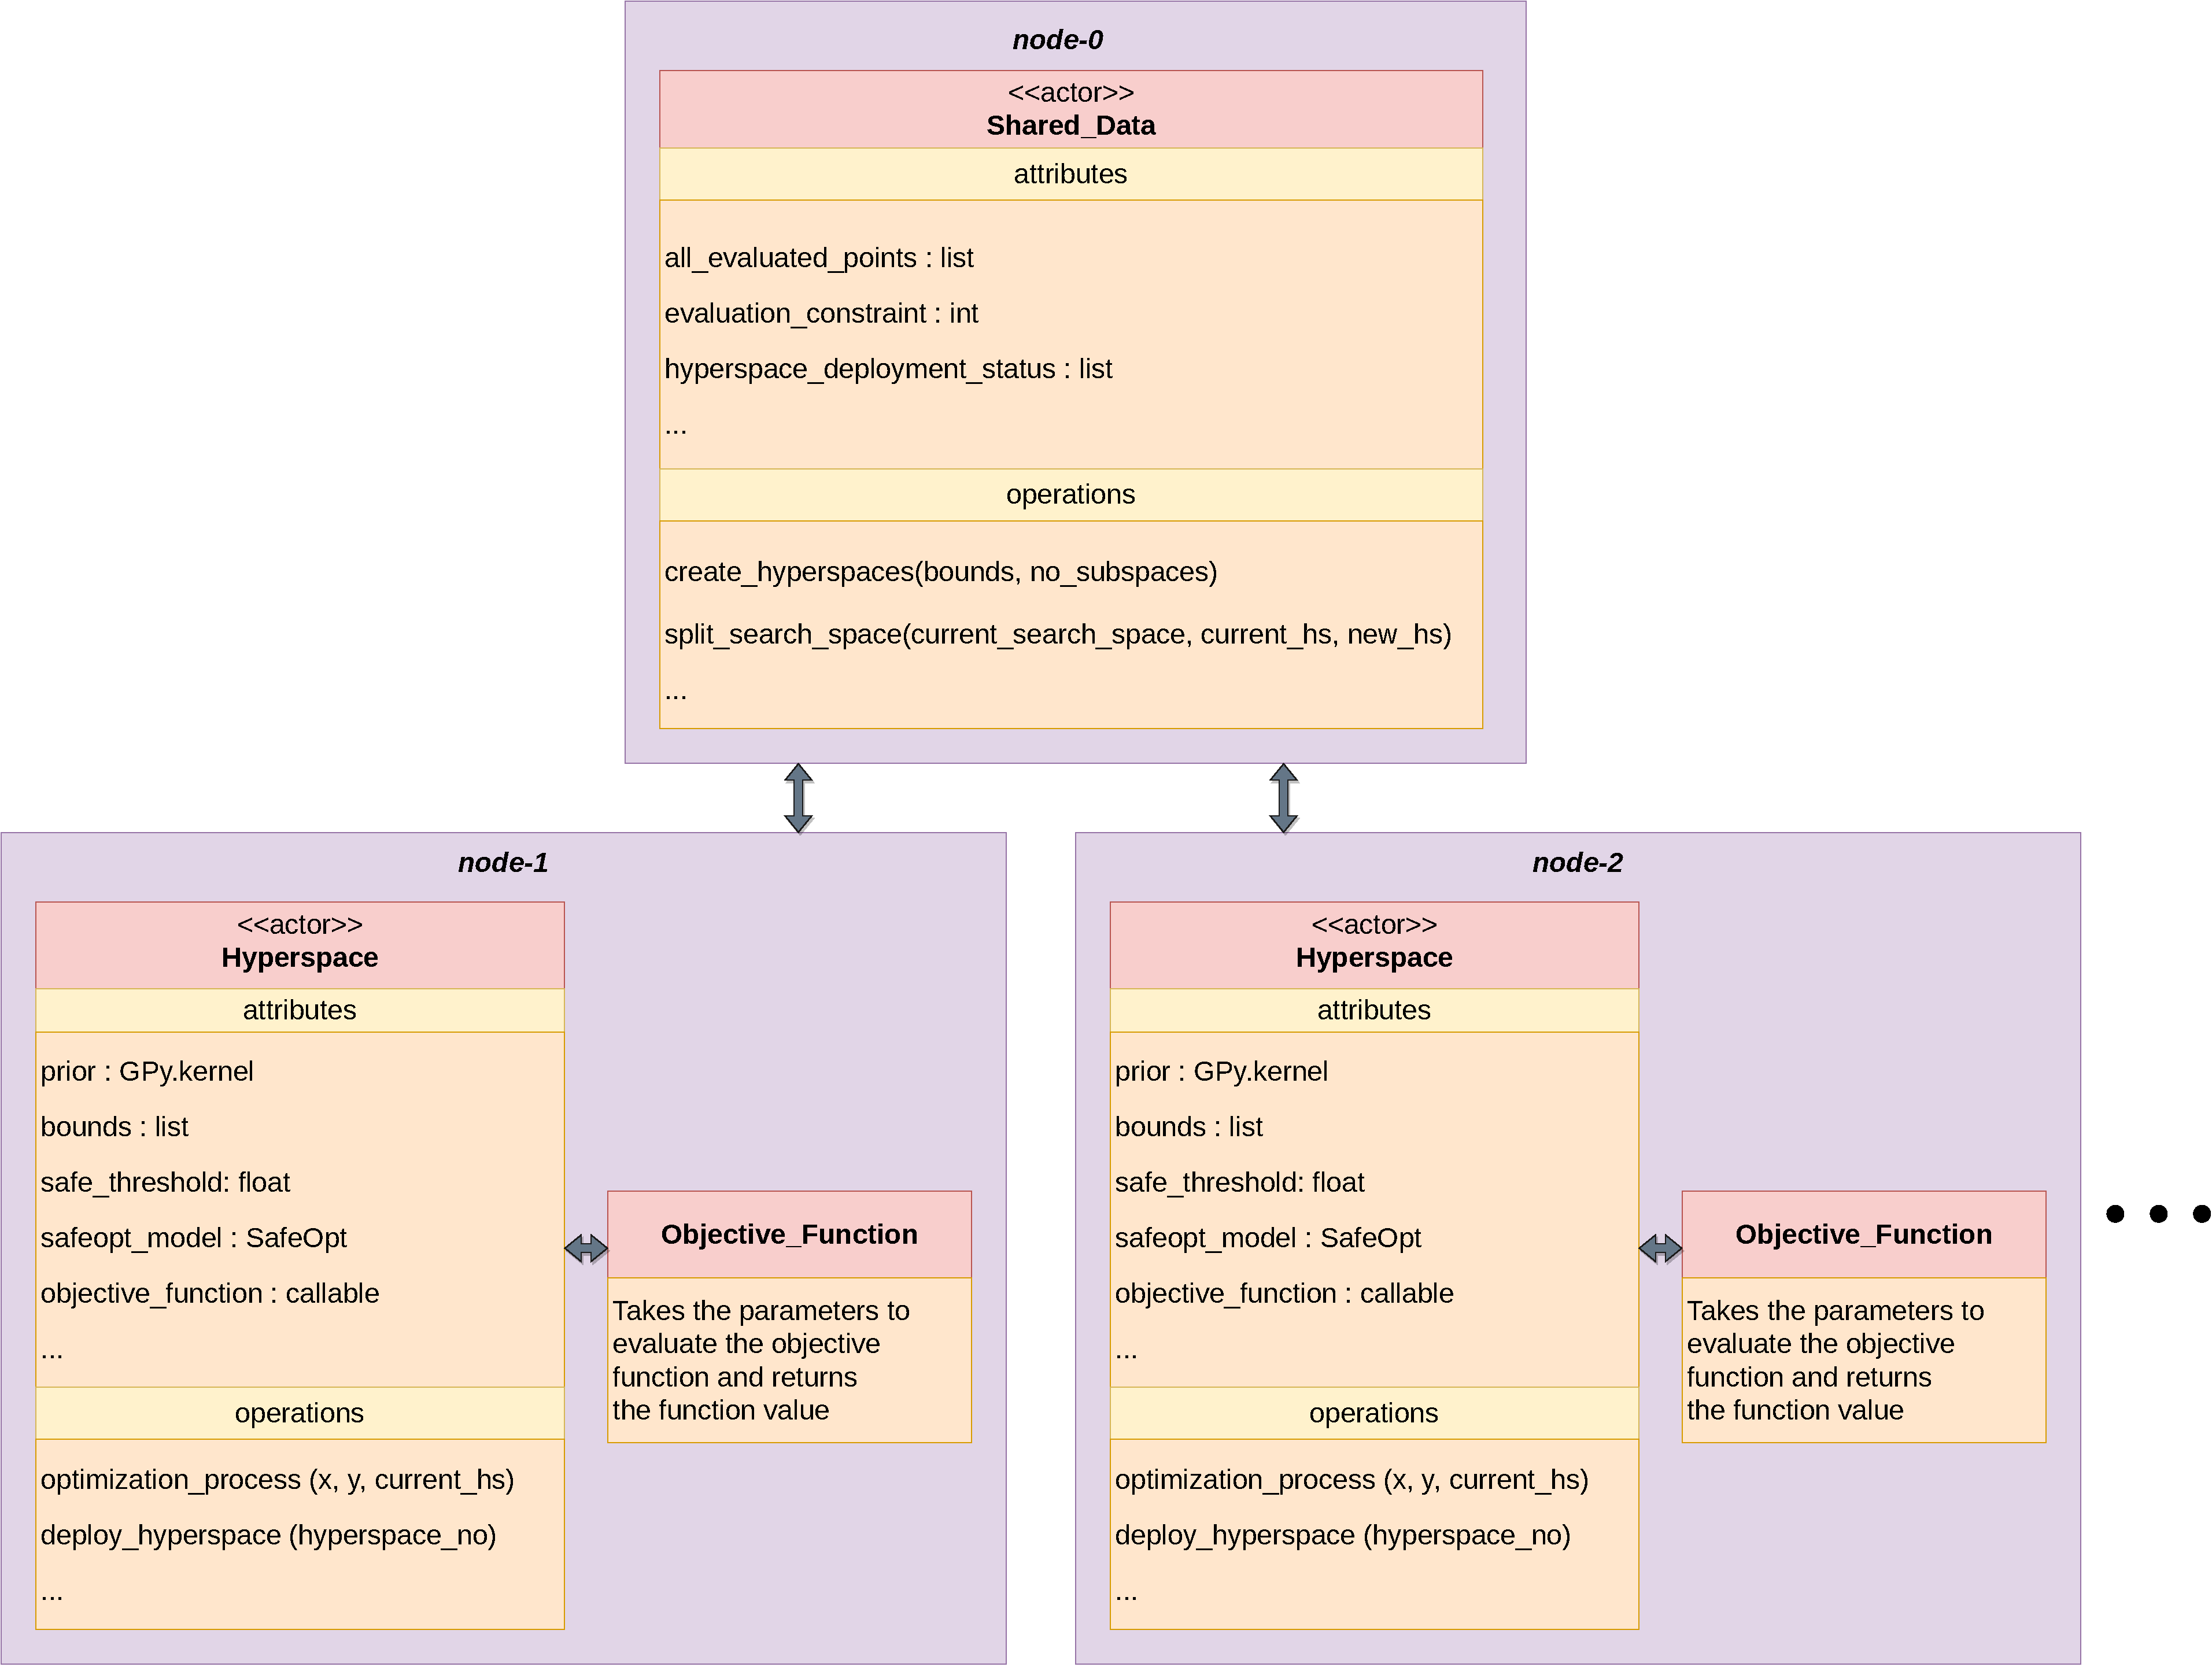
\includegraphics[scale=0.3]{figures/dbo-architecture.pdf}
	\caption{\textit{DistributedSafeOpt} Software Architecture}
	\label{fig:dsbo-architecture}
\end{figure}
Once the \textit{Shared Data} actor is created, the driver program creates a \textit{Hyperspace} actor to start the optimization process and waits for its completion to write the results to files. Point evaluated in any \textit{Hyperspace} actor during the optimization process will be shared with \textit{Shared Data} actor. 
Whenever a \textit{Hyperspace} actor evaluates a safe point in another hyperspace's search space, this actor requests the \textit{Shared Data} actor to split search space by sending its current search space bounds, current safe hyperspace number, and new hyperspace number. \textit{Hyperspace} actor will instantiate an \textit{objective function} to evaluate it at desired point. Hence we are effectively evaluating \textit{objective function} parallelly to have more number of function evaluations in a given time. 

\clearpage
\subsection{Example on creation of Hyperspaces}
\label{subsec:dsbo-example}
Figure \ref{fig:dsbo} illustrates an example for the division of search space to create hyperspaces for \texttt{DistributedSafeOpt} algorithm. In this example, we consider optimizing a 2-dimensional objective function, as shown in figure \ref{fig:dsbo-a}. $x1$ and $x2$ are the two search dimensions, and we are dividing each search dimension into two subspaces and then taking all possible combinations to create four hyperspaces, namely HS1, HS2, HS3, and HS4, as shown in figure \ref{fig:dsbo-b}. 

We start the optimization process from a safe point in hyperspace HS1, as shown in figure \ref{fig:dsbo-c}, and the next sampled safe point belongs to hyperspace HS3, as shown in figure \ref{fig:dsbo-d}. Since the hyperspaces differ along search dimension $x1$, we divide the search space in that direction itself to create two new search spaces, as shown in figure \ref{fig:dsbo-e}. Then the search space containing the new hyperspace HS3 will be deployed into the new computing node for the optimization process.
Furthermore, the current node optimization process over search space containing the initial hyperspace HS1 will be updated to new bounds. 

The newly deployed search space (containing hyperspaces HS3 and HS4), as shown in figure \ref{fig:dsbo-f} samples the next safe point in hyperspace HS4, splitting the search space into two leaf hyperspaces HS3 and HS4, as shown in figure \ref{fig:dsbo-g}. We will not be further splitting the leaf hyperspace.

\begin{figure}[H]
	\centering
	\begin{subfigure}{0.95\textwidth}
		\centering
		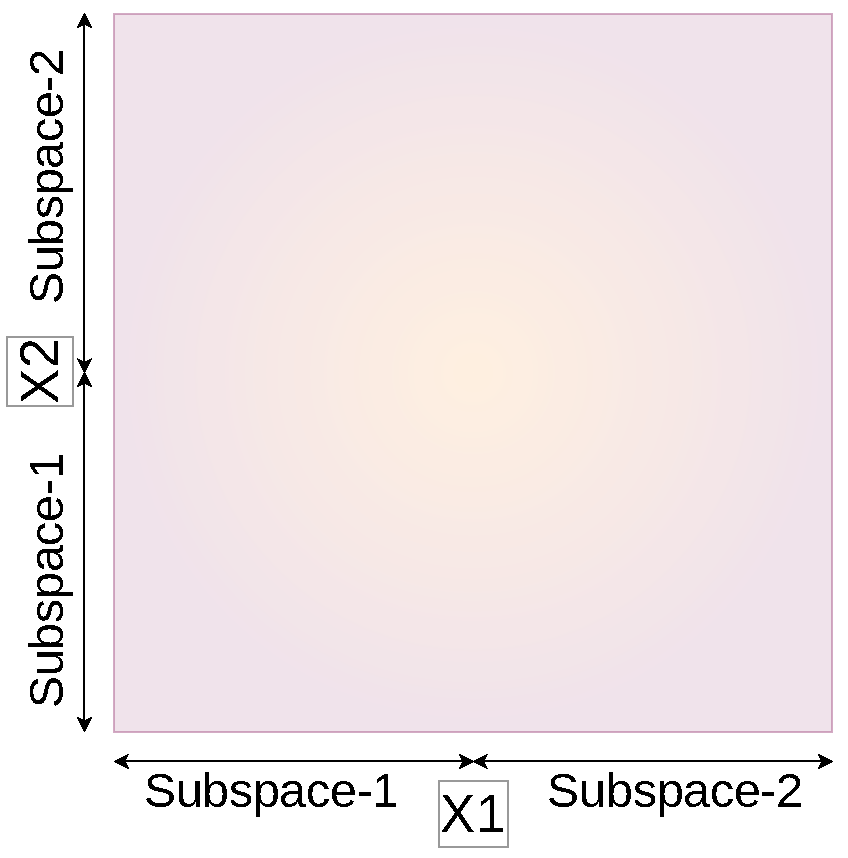
\includegraphics[scale=0.33]{figures/dbo/dbo-01.pdf}
		\caption{}
		\label{fig:dsbo-a}
	\end{subfigure}
	%	\hfill
	\begin{subfigure}{0.45\textwidth}
		\centering
		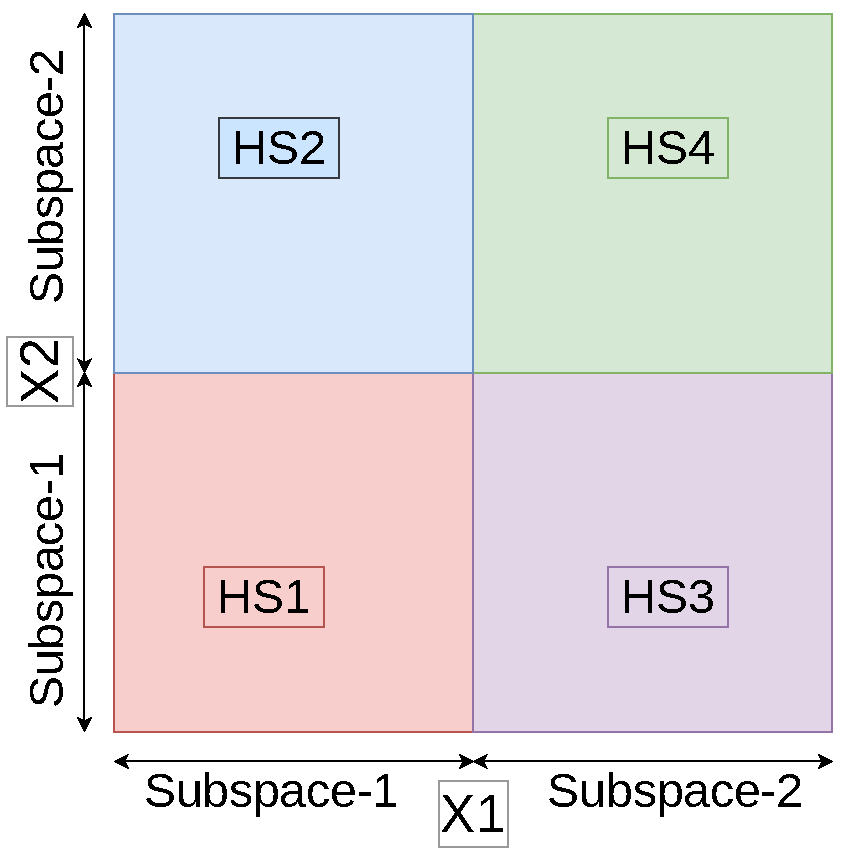
\includegraphics[scale=0.33]{figures/dbo/dbo-02.pdf}
		\caption{}
		\label{fig:dsbo-b}
	\end{subfigure}
	\begin{subfigure}{0.45\textwidth}
		\centering
		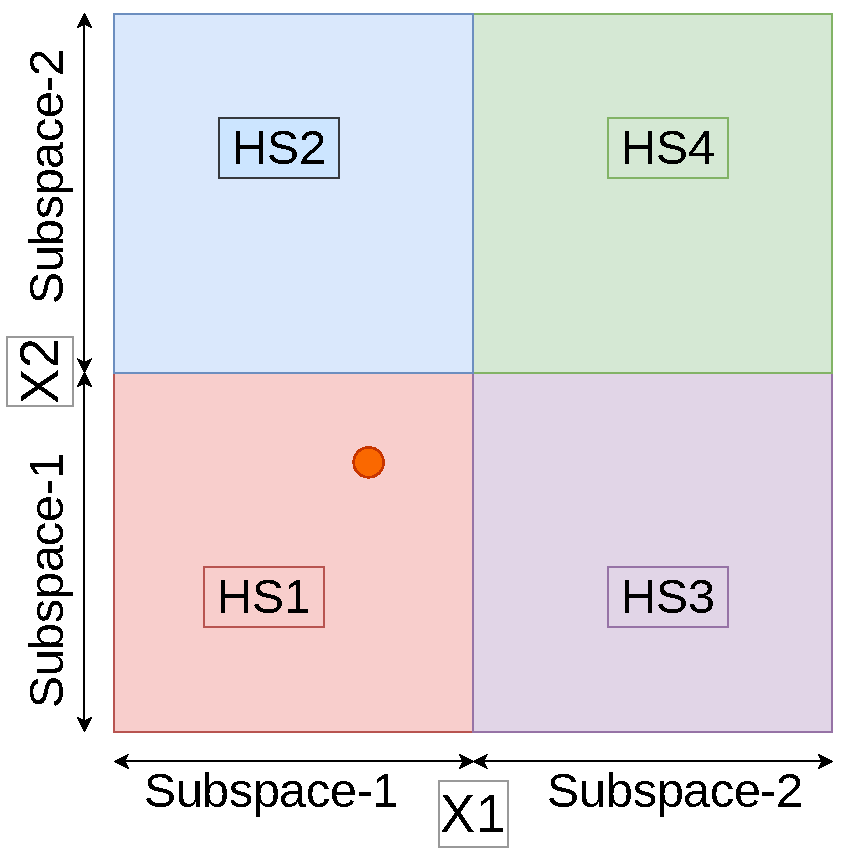
\includegraphics[scale=0.33]{figures/dbo/dbo-03.pdf}
		\caption{}
		\label{fig:dsbo-c}
	\end{subfigure}
	\begin{subfigure}{0.45\textwidth}
		\centering
		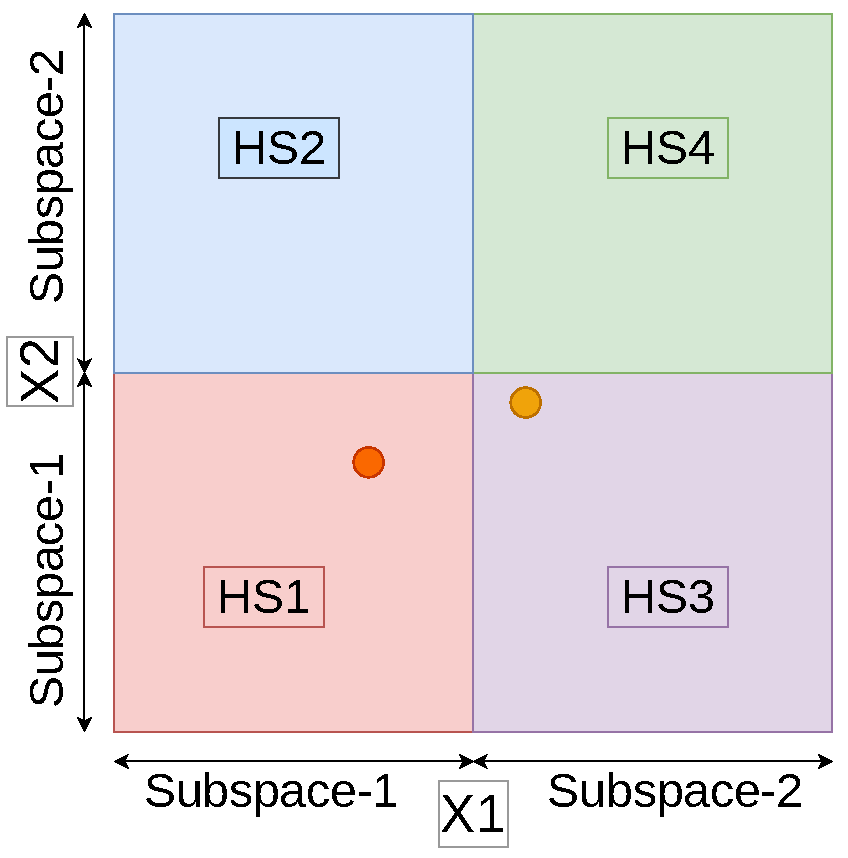
\includegraphics[scale=0.33]{figures/dbo/dbo-04.pdf}
		\caption{}
		\label{fig:dsbo-d}
	\end{subfigure}
	\begin{subfigure}{0.45\textwidth}
		\centering
		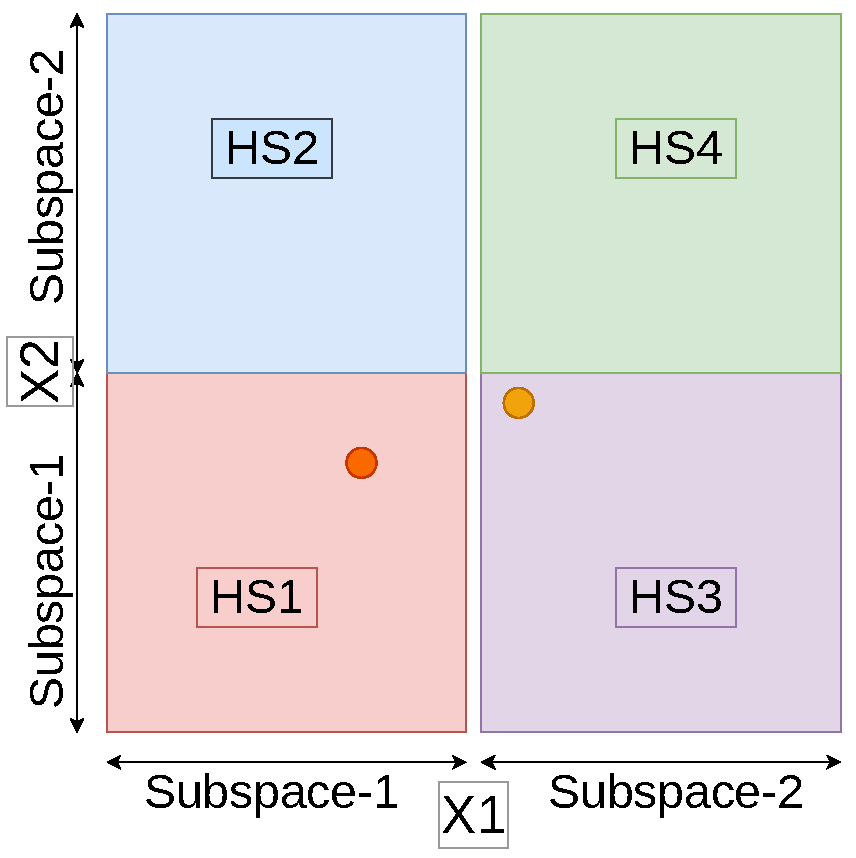
\includegraphics[scale=0.33]{figures/dbo/dbo-05.pdf}
		\caption{}
		\label{fig:dsbo-e}
	\end{subfigure}
	%	\hfill
	\begin{subfigure}{0.45\textwidth}
		\centering
		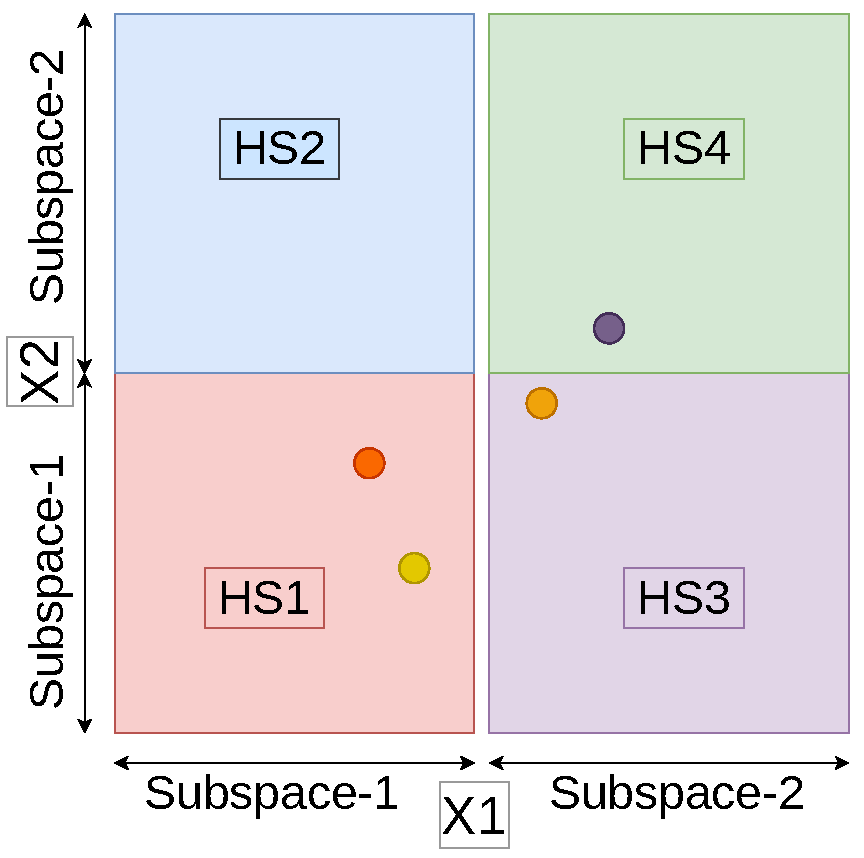
\includegraphics[scale=0.33]{figures/dbo/dbo-06.pdf}
		\caption{}
		\label{fig:dsbo-f}
	\end{subfigure}
	\begin{subfigure}{0.45\textwidth}
		\centering
		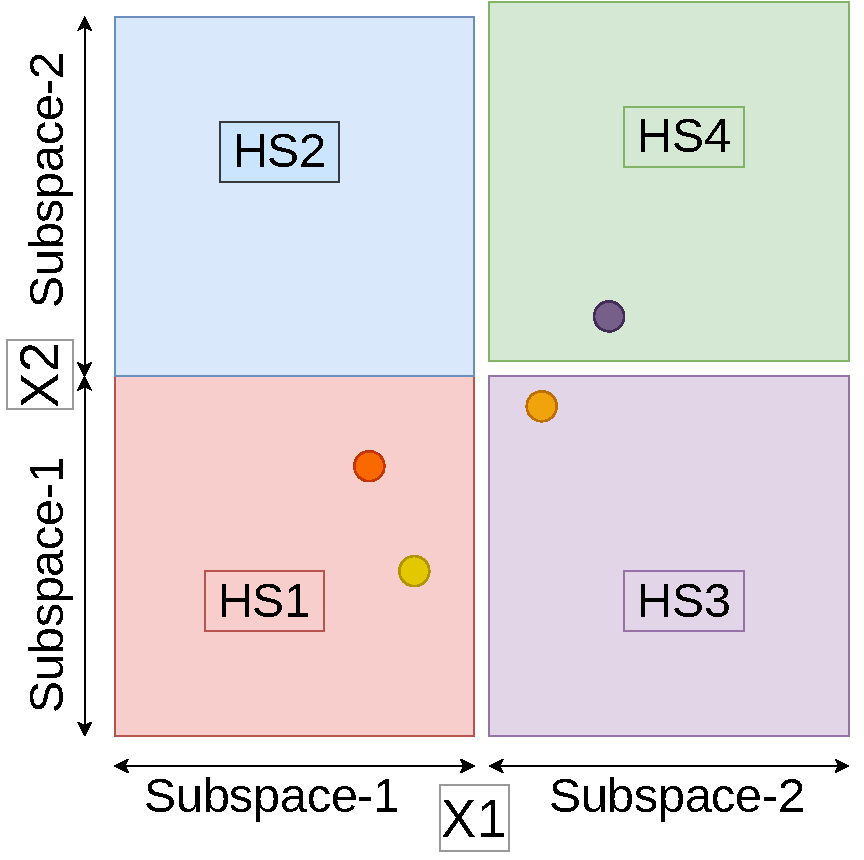
\includegraphics[scale=0.33]{figures/dbo/dbo-07.pdf}
		\caption{}
		\label{fig:dsbo-g}
	\end{subfigure}
	\caption{Illustration of \textit{DistributedSafeopt} on a 2-D search space.}
	\label{fig:dsbo}
\end{figure}

\section{Overlapped Distributed SafeOpt}\label{sec:ovr-dsbo}
The \texttt{OverlappedDistributedSafeOpt} is an extension of \texttt{DistributedSafeOpt} algorithm. The term \textit{overlapped} refers to the fraction of the hyperspace region that is overlapped with other hyperspace. Creating the overlapped hyperspaces and sharing the points evaluated in the overlapped region with the corresponding nodes are the two new ideas we are introducing to the previously discussed method in section \ref{sec:dsbo}. 

Algorithm \texttt{OverlappedDistributedSafeOpt} \ref{alg:deployovrhs} explains the creation and initial deployment of the optimization process for the whole search space into a single node. 
We start with the optimization objective function $f(\cdot)$ in $d$ dimensional domain with given prior beliefs in terms of Gaussian Processes GP($\mu, k$). We create the overlapped hyperspaces with a given amount of $ovr$ overlap fraction by dividing each search dimension into a given $n$ number of subspaces and taking all possible combinations. 

Initially, we deploy the optimization process in a single node with a given safe set $S_0$ by taking the hyperspace in which the safe seed point belongs as the initial hyperspace for the whole search space. As we proceed optimization process by sampling the objective function with a new point, we will check whether the point belongs to any other hyperspace. 
Suppose the point is safe and belongs to some new hyperspace. In that case, \texttt{DeployOverlappedHyperspace} \ref{alg:deployovrhs} algorithm will instantiate a new optimization process into a new node for that hyperspace. Alternatively, if the point (safe or unsafe) belongs to the overlapped region, we will share that point with all corresponding hyperspaces.

Furthermore, we will continue to the next iteration of the optimization process in all other cases. At any time, the objective function evaluated at a given point will be added to the global array \textit{all points evaluted}. An abstract architecture of the software implementation and an example showing how hyperspaces are created is discussed in the following subsections.\\


\begin{algorithm}[H]
%	\SetAlgoVlined
	\caption{\texttt{OverlappedDistributedSafeOpt}}
	\label{alg:ovrdsbo}
	\KwIn{Objective function $f$, GP prior($\mu, k$), Domain $\mathcal{X} \subset \mathbb{R}^d$, Number of subspaces per dimension $n$, Overlap  fraction $ovr$, Safe seed set $S_0$, Safety threshold $h$, Evaluation contraint $L$}
	\ForEach{$searchDimension$ in $\mathcal{X}$}
	{
		divide $searchDimension$ into $n$ subspaces.\\
		extend the bounds of subspaces to given $ovr$ fraction.
	}
	Take all possible combinations of subspaces to form $hyperspaces$. $(n^d)$\\
	$currentSafeHyperspace = hyperspace | S_0 \in hyperspace$\\
	Initially deploy optimization process for whole search-space into a single node.\\		
\end{algorithm}

\begin{algorithm}
%	\SetAlgoVlined
	\caption{\texttt{DeployOverlappedHyperspace}}
	\label{alg:deployovrhs}
	\KwIn{$f$, GP($\mu, k$), $\mathcal{X}$, $S_0$, $h$, $L$, $currentSafeHyperspace$}
	Initialize \texttt{SafeOpt} with safe seed points $S_0$.\\
	\If{currentSafeHyperspace $is$ leafHyperspace}
	{
		\While{$L>0$}
		{
			add shared points to \texttt{SafeOpt} model\\
			$newPoint=$ \texttt{SafeOpt}.optimize()\\
			$funcValue=f(newPoint)$\\
			add $(newPoint,funcValue)$ to $S_0$\\
			\If{$newPoint$ belongs to overlapped search area}
			{
				share $newPoint$ to corresponding hyperspaces
			}
		}
		\KwRet{}
	}
	\While{$L>0$}
	{
		add shared points to \texttt{SafeOpt} model\\
		$newPoint=$ \texttt{SafeOpt}.optimize()\\
		$funcValue=f(newPoint)$\\
		add $(newPoint,funcValue)$ to $S_0$\\
		\If{$newPoint$ belongs to overlapped search area}
		{
			share $newPoint$ to corresponding hyperspaces
		}
		$newSafeHyperspace = hyperspace | newPoint \in hyperspace$\\
		\eIf{$funcValue \ge h$ \textbf{AND} $newSafeHyperspace \neq currentSafeHyperspace$}
		{
			Split the search-space between two hyperspaces into $newSearchSpace$ and $currentSearchSpace$.\\
			Call \texttt{DeployHyperspace} for $newSearchSpace$ corresponding to $newSafeHyperspace$ to new worker node.\\
			Update the current worker node's search-space to $currentSearchSpace$ corresponding to $currentSafeHyperspace$ and continue optimization process.\\
		}
		{
			add $(newPoint,funcValue)$ to \texttt{SafeOpt} model.\\
		}
	}
\end{algorithm}

\subsection{Implementation Details}\label{subsec:ovr-dsbo-impl}
The base of this algorithm's implementation is the same as the DistributedSafeOpt algorithm as discussed in subsection \ref{subsec:dsbo-impl}. Changes are made to \textit{create hyperspaces} method of \textit{Shared Data} actor class to create overlapped hyperspaces instead of non-overlapped hyperspaces, as discussed in section \ref{sec:dsbo}. We also added a new method into the \textit{Hyperspace} actor class to communicate the points evaluated in the shared region of hyperspaces. Figure \ref{fig:ovr-dsbo-architecture} shows the abstract representation of the implementation.

The overlap fraction \textit{ovr}, input to the algorithm, tells us the amount of region to take for overlap in each search dimension. We are taking all possible combinations of these overlapped subspaces to create overlapped hyperspaces. Since the search space is overlapped, the point evaluated can belong to $n^d$ hyperspaces. So in the worst case, we have to communicate an evaluated point to $n^d-1$ other nodes.

The method \textit{send shared points} in \textit{Hyperspace} actor class will communicate the evaluated point to corresponding other nodes. The node receiving the shared point will add that point to the model before sampling the new point for evaluation. Thus it reduces the possible duplicate evaluation of a point and improves the model's belief in that search area.

\begin{figure}[H]
	\centering
	\hspace*{-6em}
	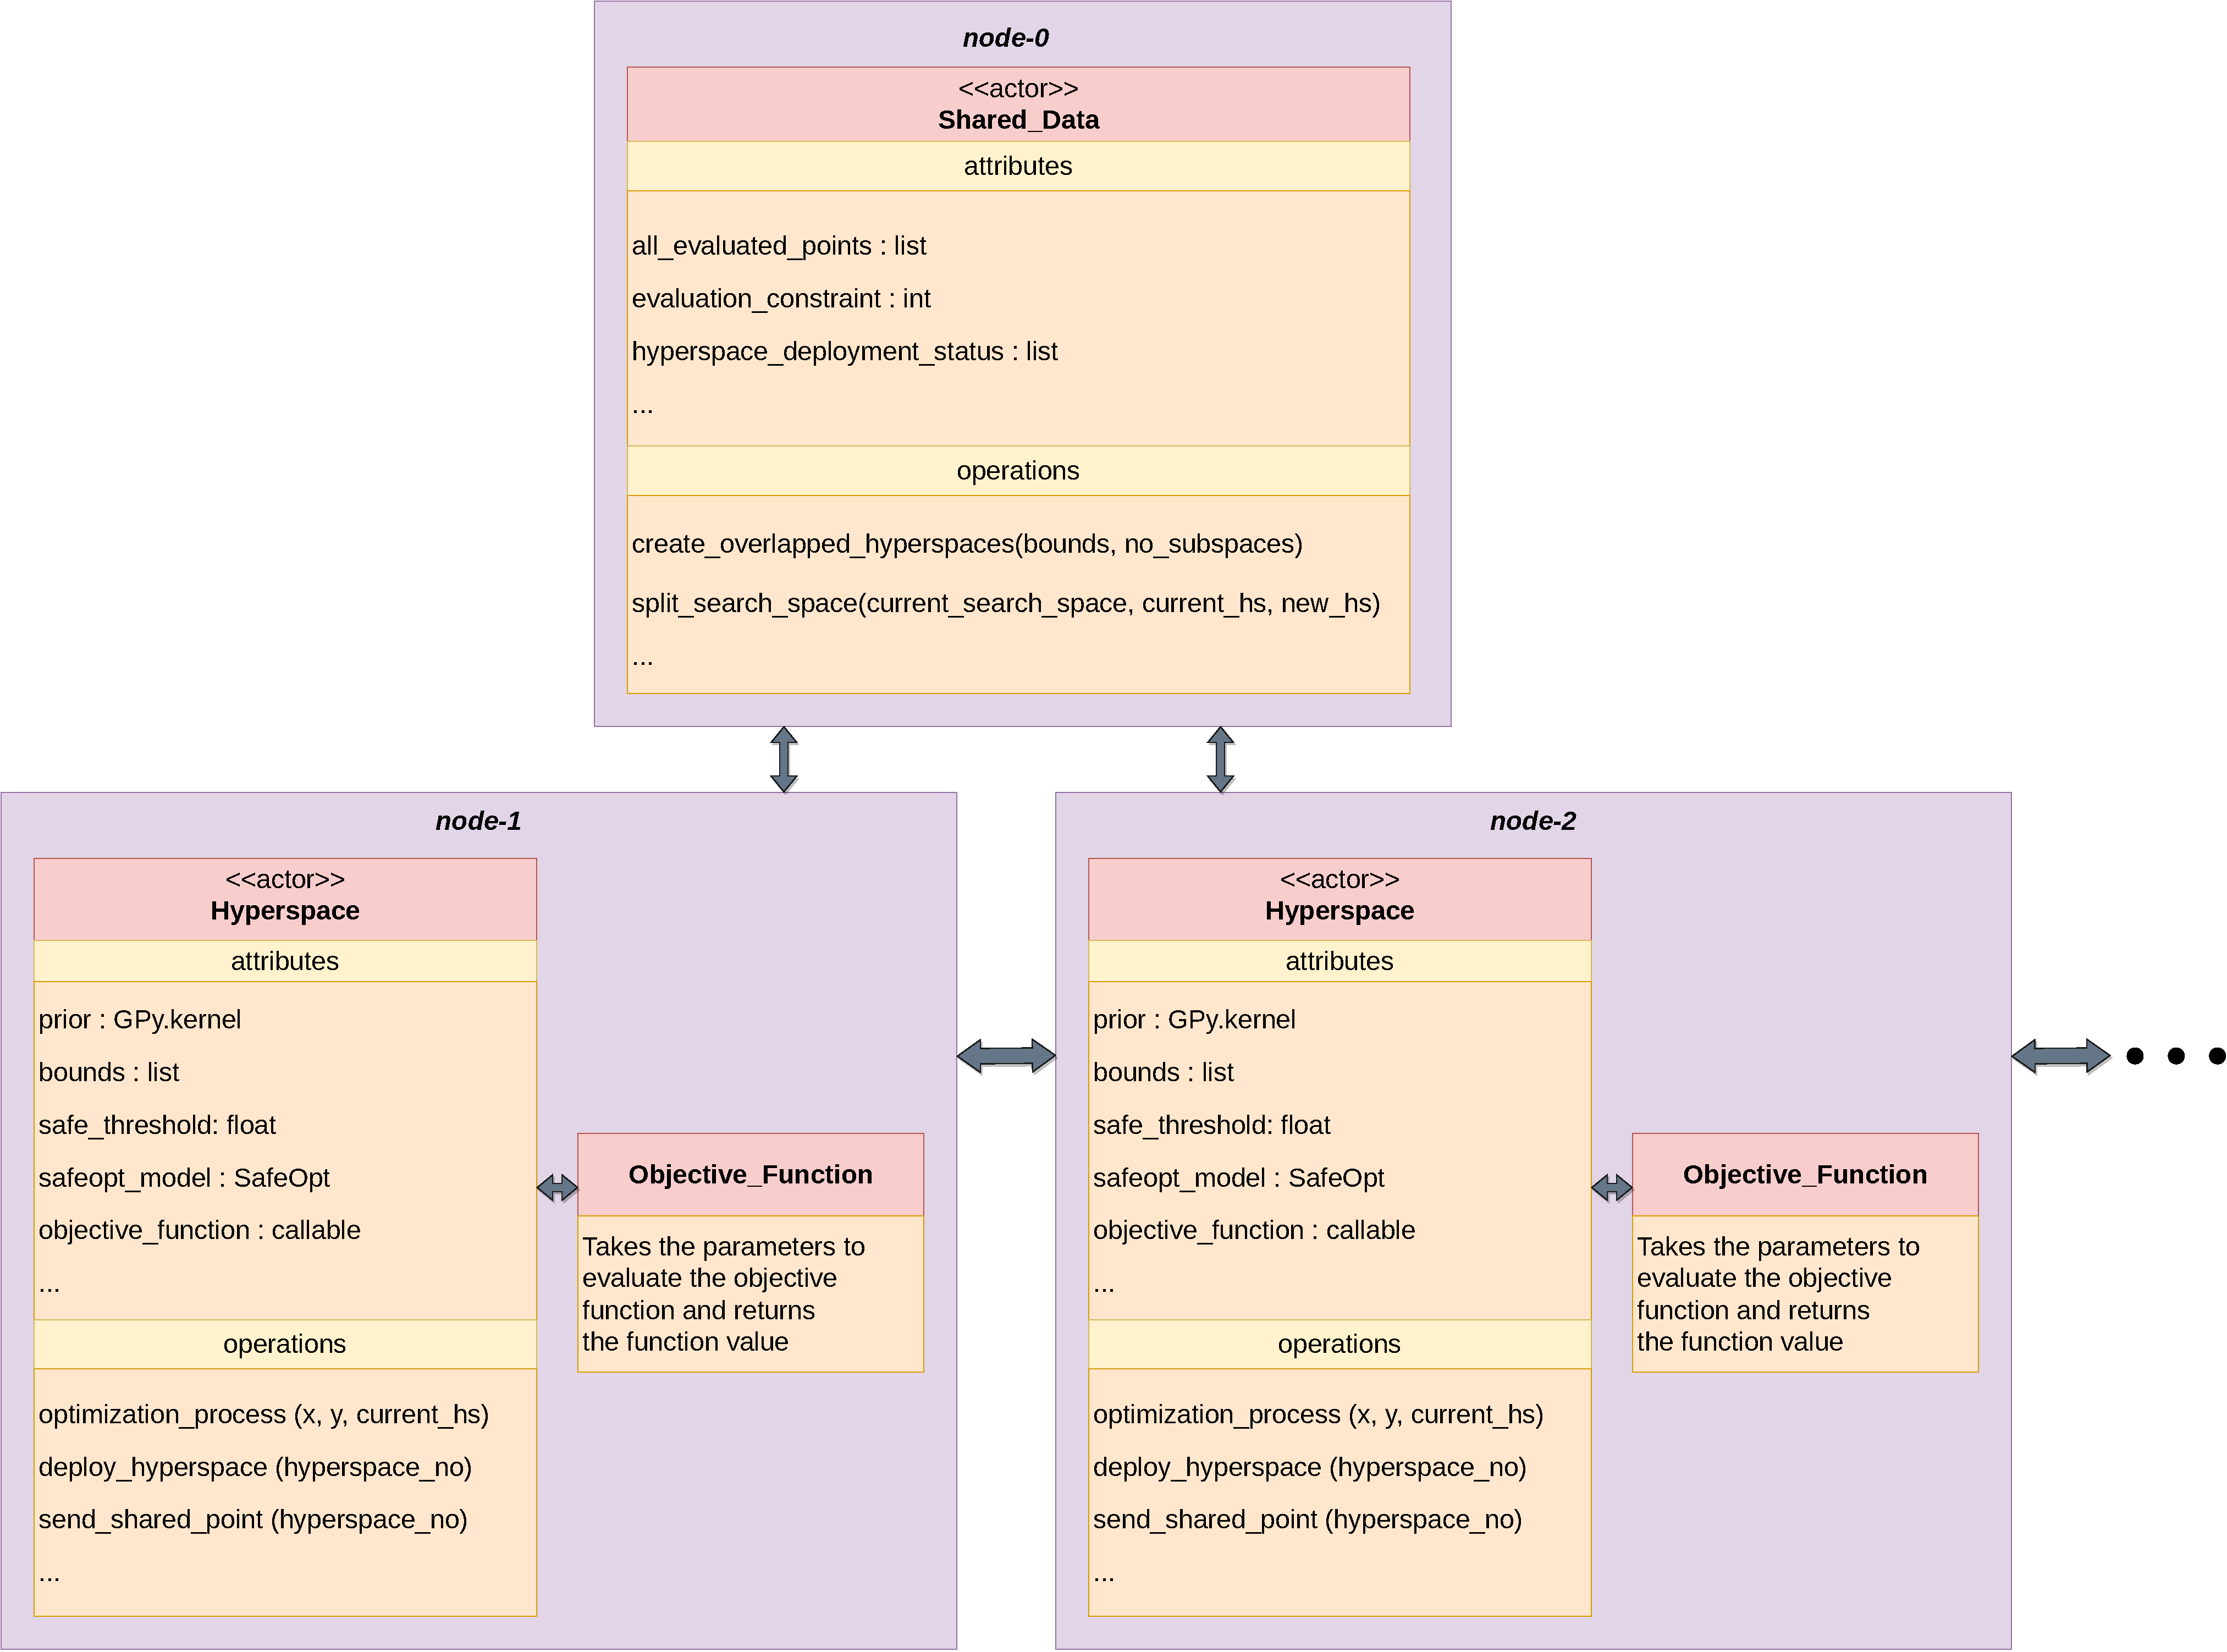
\includegraphics[scale=0.28]{figures/ovr-dbo-architecture.pdf}
	\caption{\textit{OverlappedDistributedSafeOpt} Software Architecture}
	\label{fig:ovr-dsbo-architecture}
\end{figure}

\subsection{Example on creation of Overlapped-Hyperspaces}
Figure \ref{fig:ovr-dsbo} illustrates an example for the division of search space to create hyperspaces for \texttt{OverlappedDistributedSafeOpt} algorithm. In this example, we consider optimizing a 2-dimensional objective function, as shown in figure \ref{fig:ovr-dsbo-a}. $x1$ and $x2$ are the two search dimensions, and we are dividing each search dimension into two overlapping subspaces and then taking all possible combinations to create four overlapped hyperspaces, namely HS1, HS2, HS3, and HS4, as shown in figure \ref{fig:ovr-dsbo-b}. 

We start the optimization process from a safe point in hyperspace HS1, as shown in figure \ref{fig:ovr-dsbo-c}, and the next sampled safe point belongs to hyperspace HS3, as shown in figure \ref{fig:ovr-dsbo-d}. Since the hyperspaces differ along search dimension $x1$, we divide the search space in that direction itself to create two new search spaces, as shown in figure \ref{fig:ovr-dsbo-e}. Then the search space containing the new hyperspace HS3 will be deployed into the new computing node for the optimization process.

Furthermore, the current node optimization process over the search space containing the initial hyperspace HS1 will be updated to new bounds. The search space containing overlapped hyperspaces HS1 and HS2 evaluates the new point in a region shared with HS1, so that point will be shared with another node that is optimizing in the HS1 search space.
The newly deployed search space (containing hyperspaces HS3 and HS4), as shown in figure \ref{fig:ovr-dsbo-f} samples the next safe point in hyperspace HS4, splitting the search space into two leaf hyperspaces HS3 and HS4, as shown in figure \ref{fig:ovr-dsbo-g}. We will not be further splitting the leaf hyperspace.
\begin{figure}[H]
	\centering
	\begin{subfigure}{0.95\textwidth}
		\centering
		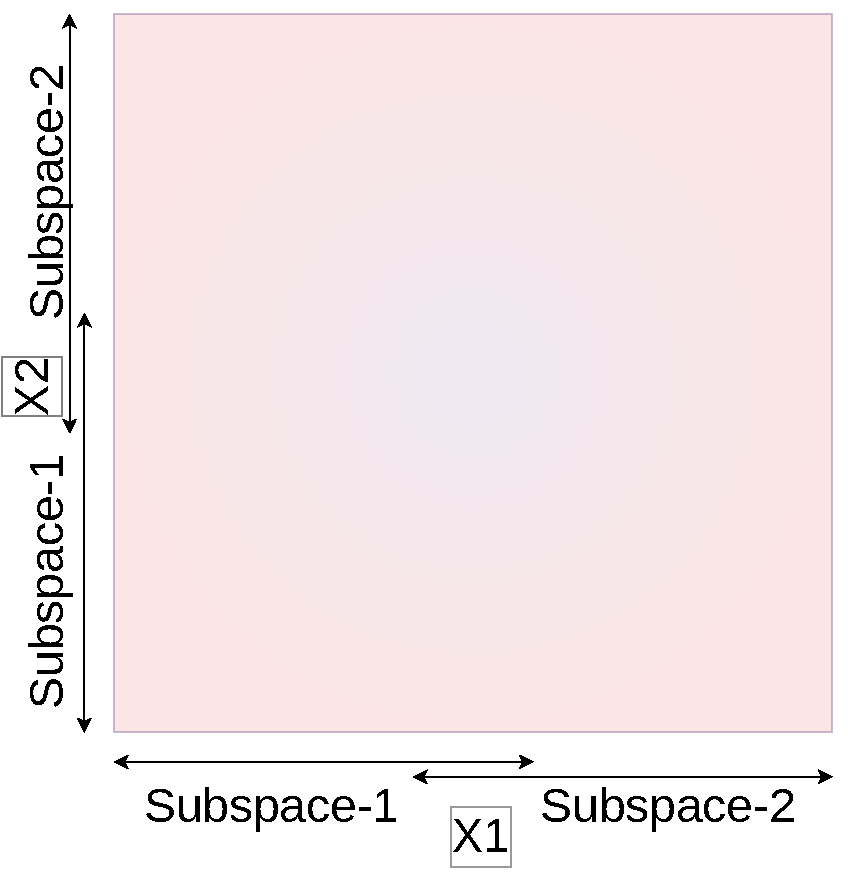
\includegraphics[scale=0.3]{figures/ovr-dbo/ovr-dbo-01.pdf}
		\caption{}
		\label{fig:ovr-dsbo-a}
	\end{subfigure}
	%	\hfill
	\begin{subfigure}{0.45\textwidth}
		\centering
		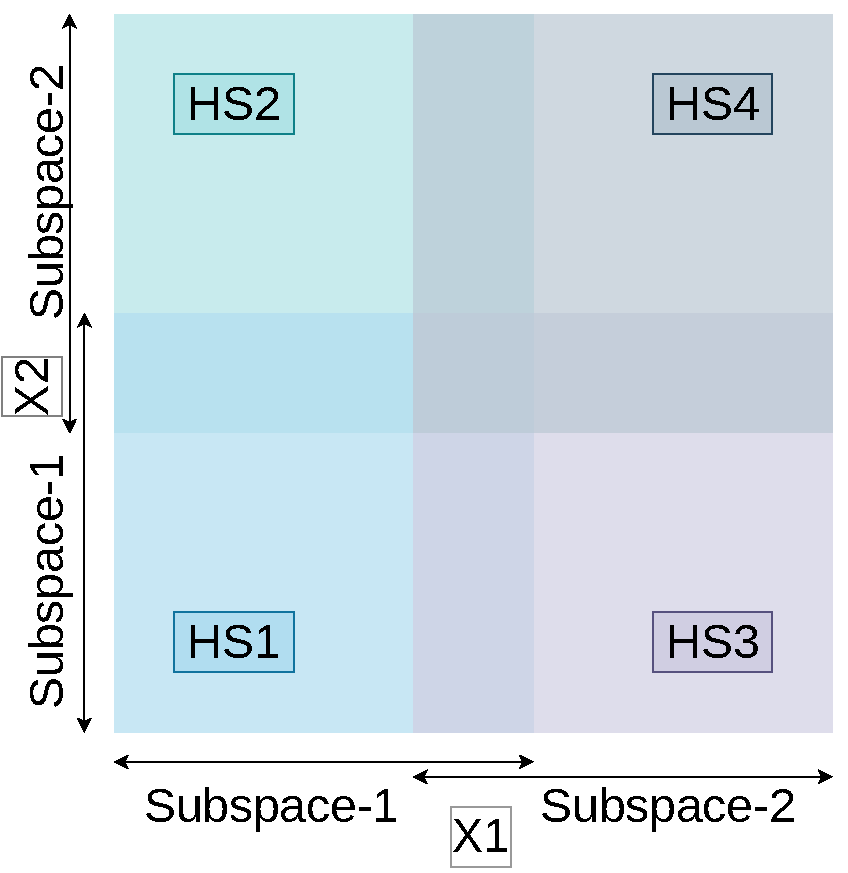
\includegraphics[scale=0.3]{figures/ovr-dbo/ovr-dbo-02.pdf}
		\caption{}
		\label{fig:ovr-dsbo-b}
	\end{subfigure}
	\begin{subfigure}{0.45\textwidth}
		\centering
		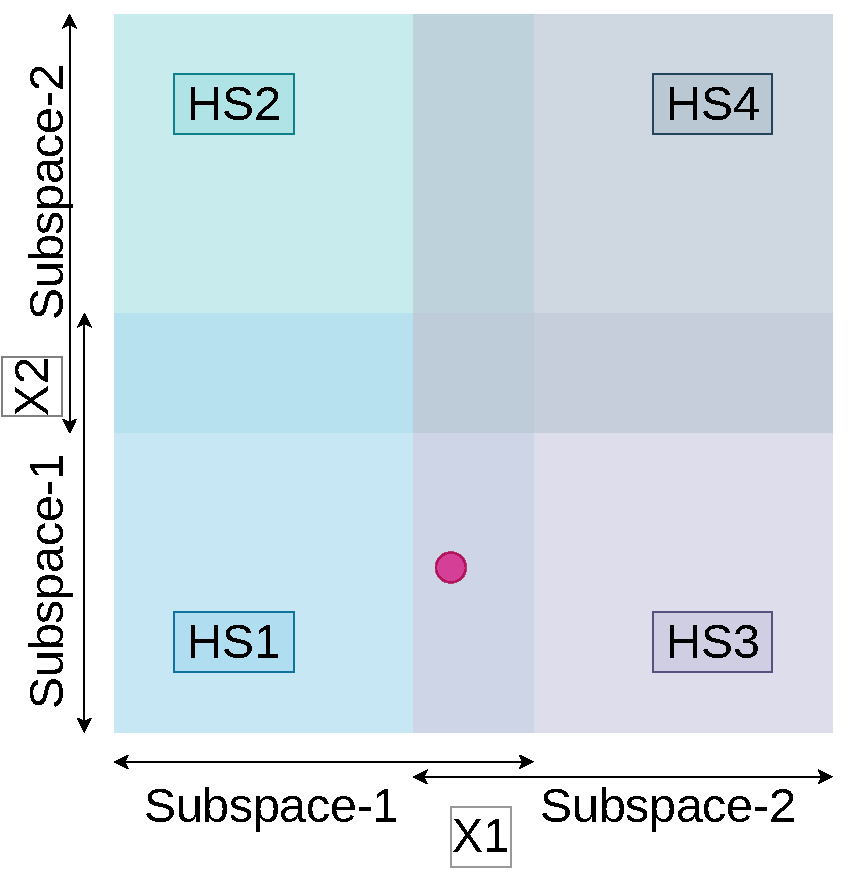
\includegraphics[scale=0.3]{figures/ovr-dbo/ovr-dbo-03.pdf}
		\caption{}
		\label{fig:ovr-dsbo-c}
	\end{subfigure}
	\begin{subfigure}{0.45\textwidth}
		\centering
		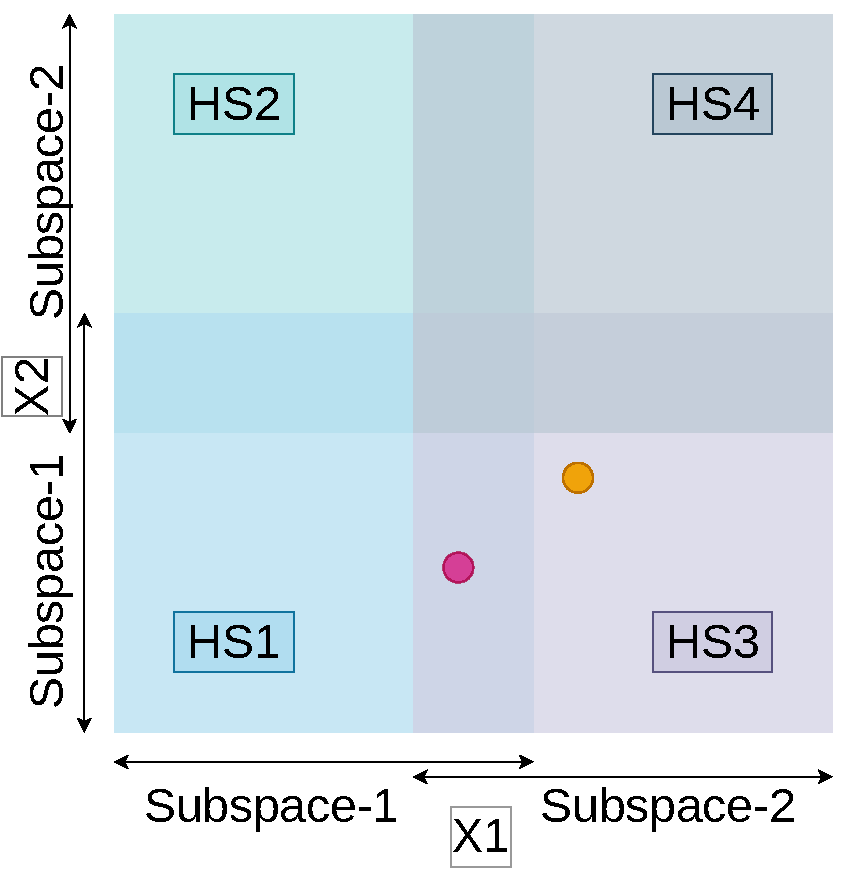
\includegraphics[scale=0.3]{figures/ovr-dbo/ovr-dbo-04.pdf}
		\caption{}
		\label{fig:ovr-dsbo-d}
	\end{subfigure}
	\begin{subfigure}{0.45\textwidth}
		\centering
		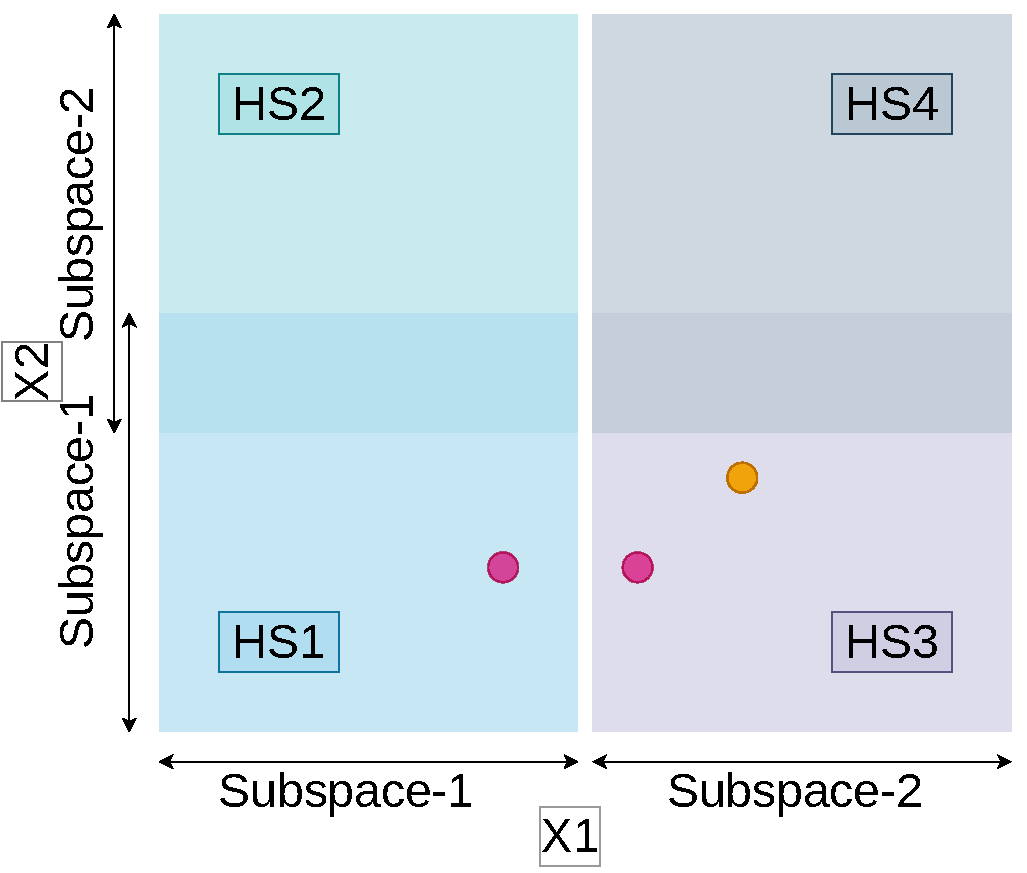
\includegraphics[scale=0.3]{figures/ovr-dbo/ovr-dbo-05.pdf}
		\caption{}
		\label{fig:ovr-dsbo-e}
	\end{subfigure}
	%	\hfill
	\begin{subfigure}{0.45\textwidth}
		\centering
		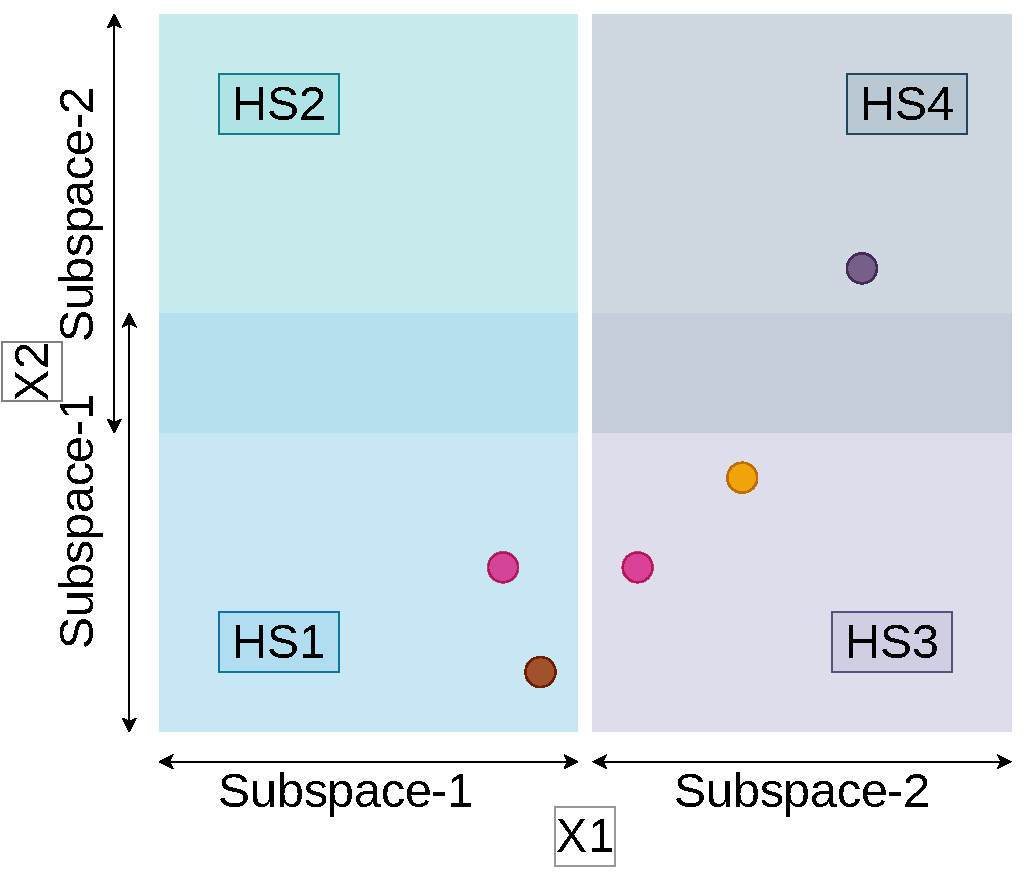
\includegraphics[scale=0.3]{figures/ovr-dbo/ovr-dbo-06.pdf}
		\caption{}
		\label{fig:ovr-dsbo-f}
	\end{subfigure}
	\begin{subfigure}{0.45\textwidth}
		\centering
		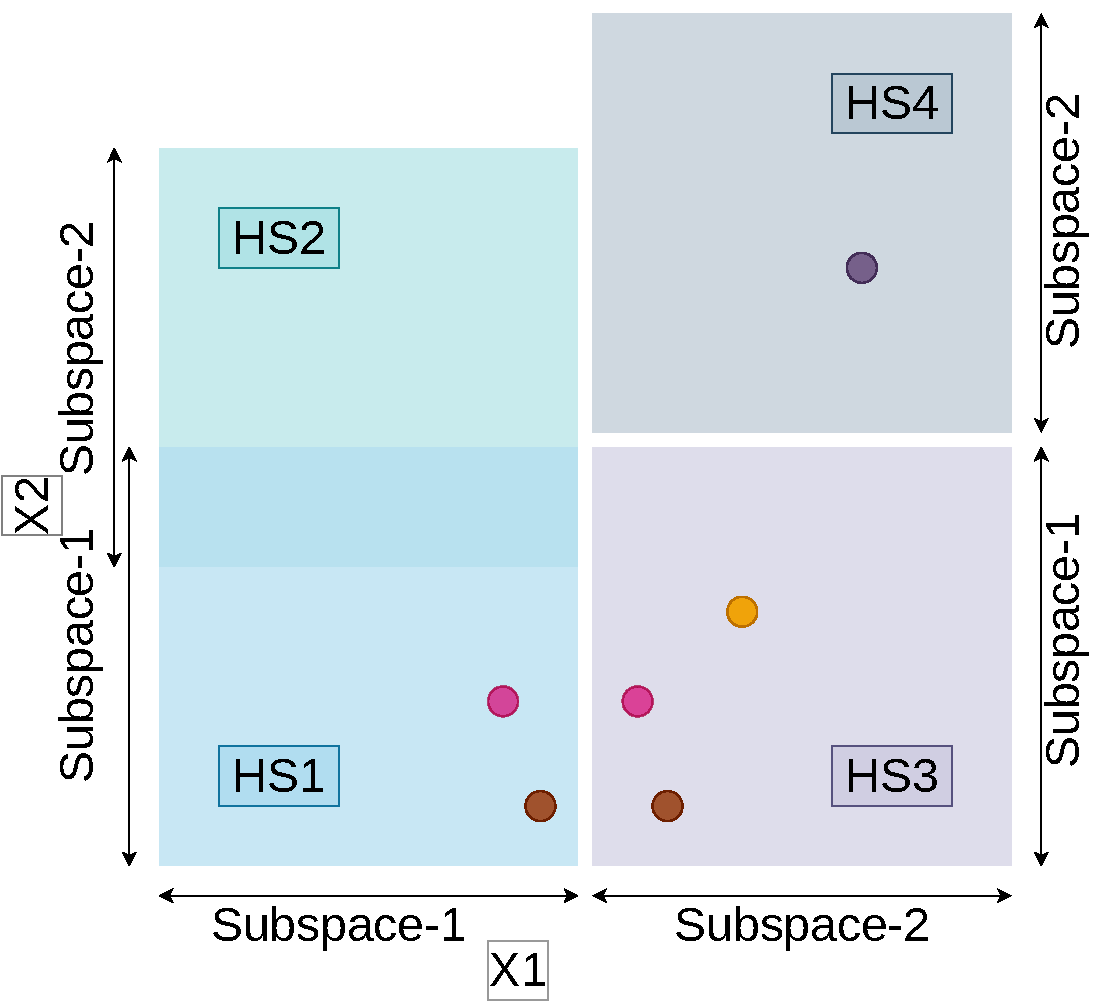
\includegraphics[scale=0.3]{figures/ovr-dbo/ovr-dbo-07.pdf}
		\caption{}
		\label{fig:ovr-dsbo-g}
	\end{subfigure}
	\caption{Illustration of \textit{OverlappedDistributedSafeOpt} on a 2-D search space}
	\label{fig:ovr-dsbo}
\end{figure}